%%%%%%%%%%%%%%%%%%%%%%%%%%%%%%%%%%%%%%%%%%%%%%%%%%%%%%%%%%%%%%%%%%%%%%
% How to use writeLaTeX: 
%
% You edit the source code here on the left, and the preview on the
% right shows you the result within a few seconds.
%
% Bookmark this page and share the URL with your co-authors. They can
% edit at the same time!
%
% You can upload figures, bibliographies, custom classes and
% styles using the files menu.
%
%%%%%%%%%%%%%%%%%%%%%%%%%%%%%%%%%%%%%%%%%%%%%%%%%%%%%%%%%%%%%%%%%%%%%%

\documentclass[12pt]{article}

\usepackage{sbc-template}

\usepackage{graphicx,url}

\usepackage{tikz}
\usetikzlibrary{arrows.meta, positioning, shapes.geometric}

%\usepackage[brazil]{babel}   
\usepackage[utf8]{inputenc}  

\usepackage{amsmath}
\sloppy

\title{Análise de Privacidade e Utilidade em LLMs Federados \\ com Ajuste Fino via LoRA}

\author{Guilherme Eduardo Silva Batalhoti\inst{1}}


\address{FCT/Unesp -- Presidente Prudente, São Paulo, Brasil
  \email{guilherme.batalhoti@unesp.br}
}

\begin{document} 

\maketitle

\begin{resumo}
Este trabalho investiga a relação entre descentralização de dados e riscos de memorização em Large Language Models (LLMs) submetidos a fine-tuning via Aprendizado Federado, utilizando o modelo TinyLlama-1.1B-Chat com adaptadores LoRA. Para avaliar o impacto da fragmentação dos dados, foram simulados três cenários federados (K = 2, 4, 6) com treinamento no dataset Alpaca-GPT4, analisando a fidelidade estrutural e semântica das respostas por meio de Exact Match, distância de Levenshtein e similaridade de cosseno. Os resultados mostram ausência de memorização literal em todos os cenários, reforçando a segurança textual do método, enquanto a qualidade semântica das respostas permanece estável ou ligeiramente superior em ambientes mais fragmentados, sugerindo que a diversidade de clientes atua como regularizador. O estudo confirma a viabilidade do fine-tuning federado para reduzir riscos de vazamento sem comprometer a utilidade do modelo e abre caminho para investigações futuras com técnicas avançadas de agregação e privacidade diferencial.
\end{resumo}


\section{Introdução} \label{sec:introdução}

O avanço recente da Inteligência Artificial (IA) tem sido impulsionado por modelos treinados em grandes conjuntos de dados (\textit{datasets}), ao mesmo tempo em que cresce a preocupação com a privacidade das informações utilizadas \cite{yurdem_federated_2024}. O treinamento tradicional de modelos de \textit{Machine Learning} (ML) em ambientes centralizados apresenta riscos éticos e regulatórios, especialmente diante de legislações como a Lei Geral de Proteção de Dados (LGPD) \cite{brasil_lei_2008}. Nesse contexto, o Aprendizado Federado (\textit{Federated Learning} – FL) surge como uma abordagem promissora ao permitir o treinamento colaborativo de modelos sem a necessidade de compartilhamento direto dos dados \cite{mcmahan_communication-efcient_2017}, \cite{beutel_flower_2020}.

Em paralelo, os \textit{Large Language Models} (LLMs) consolidaram-se como uma das mais poderosas aplicações de IA, apresentando desempenho notável em tarefas de Processamento de Linguagem Natural (PLN) \cite{guo_can_2025}. A adaptação desses modelos a domínios específicos, por meio do \textit{fine-tuning}, é uma prática amplamente adotada, mas que também amplifica os riscos de exposição de informações sensíveis presentes nos dados de treinamento \cite{guo_can_2025}.

A integração entre FL e LLMs representa uma alternativa estratégica para possibilitar o \textit{fine-tuning} de grandes modelos em ambientes descentralizados, conciliando desempenho e privacidade \cite{fajardo_fedrag_2025}, \cite{hatfaludi_foundational_2025}. Contudo, essa combinação introduz novos desafios técnicos, como a sobrecarga de comunicação e potenciais vazamentos de dados durante o processo federado. Diante disso, este trabalho investiga mecanismos de adaptação eficiente e segura de LLMs em contextos federados, com foco na mitigação de riscos de privacidade e vazamento de informações.

\section{Objetivos} \label{sec:objetivos}

O objetivo central deste artigo é avaliar a capacidade de memorização literal e semântica de LLMs em um cenário federado, variando o grau de fragmentação dos dados ($K \in {2,4,6}$) e aplicando métricas de similaridade estrutural e semântica sob um protocolo de inferência determinístico

\section{Fundamentação Teórica} \label{sec:fundamentação}

\subsection{Aprendizado Federado (FL)} \label{subsec:fedLearning}

O Aprendizado Federado é um paradigma de aprendizado distribuído que permite treinar modelos de forma colaborativa sem centralizar os dados \cite{mcmahan_communication-efcient_2017, beutel_flower_2020}. Nesse processo, cada cliente treina localmente com seus próprios dados e envia apenas as atualizações ao servidor, que realiza a agregação para compor o modelo global, como ilustrado na Figura \ref{fig:exeploFL}.

\begin{figure}[ht]
\centering
\includegraphics[width=.9\textwidth]{img/FedLearning.png}
\caption{Exemplo de arquitetura de FL. Fonte: autor.}
\label{fig:exeploFL}
\end{figure}

Essa abordagem reduz problemas de “silos de dados” \cite{hatfaludi_foundational_2025} e utiliza, principalmente, o algoritmo \textit{Federated Averaging} (FedAvg), que realiza a média ponderada das atualizações dos clientes. A atualização do modelo global $w$ na rodada $t+1$ é dada por:

\begin{equation}
w_{t+1} = \sum_{k=1}^{K} \frac{n_k}{n} w_{t+1}^{(k)}
\label{eq:fedavg}
\end{equation}

onde $K$ é o número de clientes, $w_{t+1}^{(k)}$ são os pesos locais, $n_k$ o número de amostras de cada cliente e $n = \sum_{k=1}^{K} n_k$ o total de amostras.

Apesar de suas vantagens, o FL enfrenta desafios como heterogeneidade de dispositivos e dados \cite{li_federated_2018, wu_personalized_2020}. Além disso, sua garantia de privacidade é limitada: atualizações de modelo podem revelar informações sensíveis por meio de ataques de inferência ou reconstrução \cite{guo_can_2025}.

\subsection{LLMs, Ajuste Fino e o Risco de Privacidade}

Os Modelos de Linguagem de Grande Porte (LLMs) são modelos de IA, baseados em arquiteturas de fundação e aprendizado autossupervisionado, que se destacam pela capacidade de processar e gerar texto de forma autorregressiva \cite{patil_review_2024}. Embora pré-treinados em vastos volumes de dados genéricos da web, seu conhecimento torna-se especializado para tarefas de domínio (como medicina ou direito) através do Ajuste Fino (\textit{Fine-Tuning}).

O Ajuste Fino é um treinamento supervisionado em um conjunto de dados menor e especializado, usando técnicas como o Ajuste Fino Eficiente em Parâmetros (PEFT), para adaptar o modelo a uma tarefa específica \cite{anisuzzaman_fine-tuning_2025}.

É precisamente nesses dados de ajuste fino que reside o maior risco de privacidade. Os conjuntos de dados usados para especialização (SFT, PEFT) são frequentemente proprietários, sensíveis ou contêm informações de identificação pessoal (PII) — por exemplo, registros médicos, dados financeiros ou dados de usuários para personalização. A centralização desses dados para o ajuste fino tradicional é, portanto, impraticável ou ilegal.

Como os LLMs possuem uma capacidade elevada de memorização, as vulnerabilidades de vazamento de dados através dos gradientes (mencionadas na Seção \ref{subsec:fedLearning}) tornam-se ainda mais críticas, capazes de expor textualmente os dados sensíveis usados no treinamento \cite{guo_can_2025}.

\subsection{Métricas de Avaliação e Privacidade}

A distinção entre generalização útil e memorização de dados sensíveis em LLMs requer uma avaliação multidimensional que combine métricas estruturais, sintáticas e semânticas. O \textbf{Exact Match (EM)} atua como indicador primário de memorização \textit{verbatim}, detectando reproduções literais dos dados de treino, conforme demonstrado por \cite{carlini2021}. A métrica é definida como:

\begin{equation}
EM(\hat{Y}, Y) =
\begin{cases}
1, & \text{se } \hat{Y} = Y \\
0, & \text{caso contrário}
\end{cases}
\end{equation}

Para capturar variações mínimas que impedem o EM, emprega-se a \textbf{Distância de Levenshtein normalizada} \cite{levenshtein1966}, capaz de identificar quase-duplicatas mediante penalização de edições de caracteres. Essa similaridade estrutural é representada por:
\begin{equation}
S_{Lev}(\hat{Y}, Y) = 1 - \frac{\text{dist}(\hat{Y}, Y)}{\max(| \hat{Y} |, | Y |)}
\end{equation}
\noindent onde $\text{dist}$ denota a distância de edição e $|\cdot|$ o comprimento das cadeias.

Como complemento semântico, utiliza-se a \textbf{Similaridade de Cosseno} aplicada sobre \textit{embeddings} vetoriais (SBERT) \cite{reimers2019}, que permite aferir equivalência de significado mesmo quando não há sobreposição lexical significativa \cite{reimers2019}. Essa métrica é definida por:
\begin{equation}
S_{Sem} = \cos(\theta) = \frac{v_{\hat{Y}} \cdot v_{Y}}{|v_{\hat{Y}}| |v_{Y}|}
\end{equation}
onde os vetores $v$ são obtidos por um modelo de \textit{embedding} auxiliar (\texttt{all-MiniLM-L6-v2}).

\section{Metodologia}

Para investigar a capacidade de retenção de informação e a fidelidade de reprodução de \textit{Large Language Models} (LLMs) num contexto de instruções complexas, esta metodologia propõe uma análise quantitativa baseada na comparação direta entre as saídas geradas pelo modelo e o ``gabarito'' (\textit{ground truth}) proveniente do conjunto de dados. A Figura \ref{fig:metodologia} ilusta o passo a passo da metodologia seguida.

\begin{figure}[h]
\centering
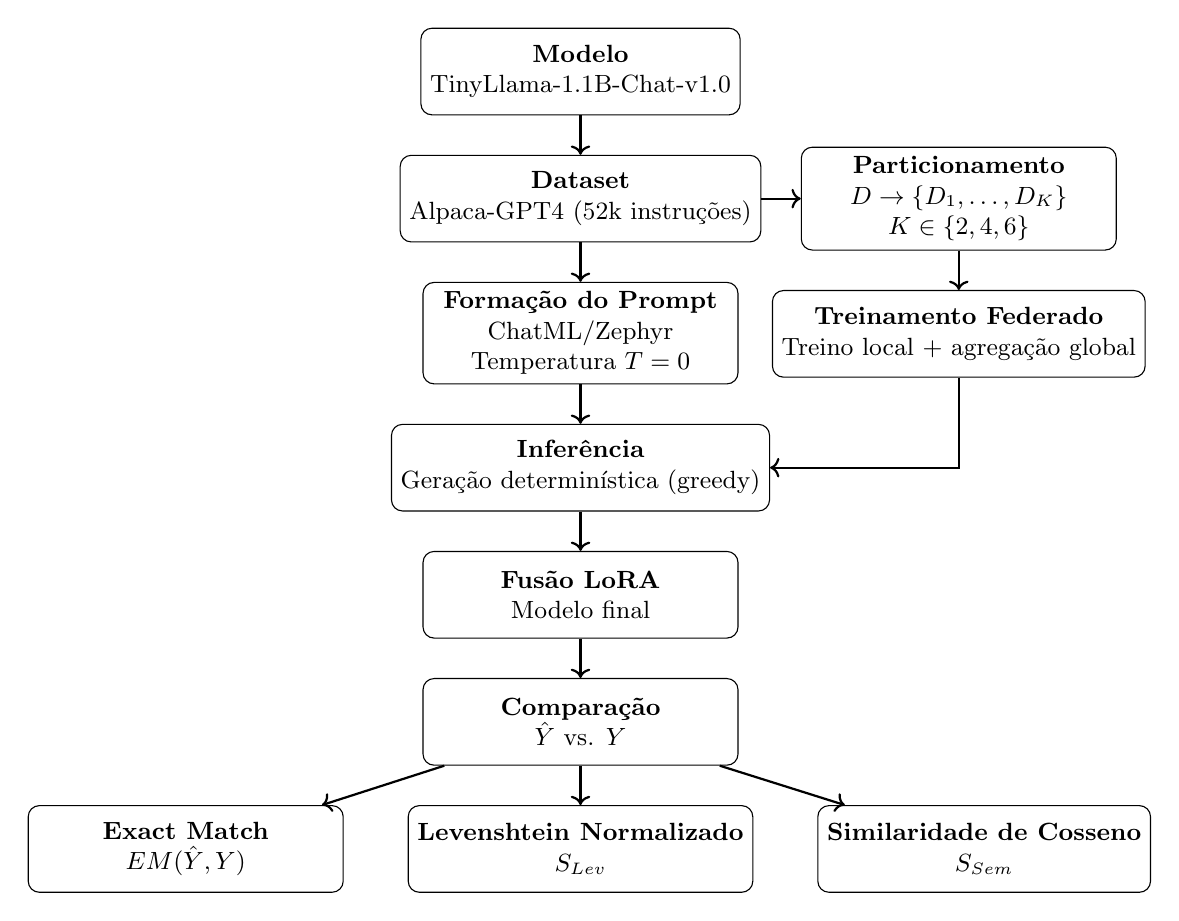
\begin{tikzpicture}[
    node distance=1.8cm,
    every node/.style={font=\small},
    proc/.style={rectangle, rounded corners, draw, align=center, minimum width=4cm, minimum height=1.1cm},
    arrow/.style={->, thick}
]

% Main flow
\node[proc] (model) {\textbf{Modelo}\\ TinyLlama-1.1B-Chat-v1.0};
\node[proc, below=.5cm of model] (dataset) {\textbf{Dataset}\\Alpaca-GPT4 (52k instruções)};
\node[proc, right=.5cm of dataset] (part) {\textbf{Particionamento}\\$D \rightarrow \{D_1, \dots, D_K\}$\\$K \in \{2,4,6\}$};
\node[proc, below=.5cm of part] (fl) {\textbf{Treinamento Federado}\\Treino local + agregação global};

\node[proc, below=.5cm of dataset] (prompt) {\textbf{Formação do Prompt}\\ChatML/Zephyr\\Temperatura $T=0$};
\node[proc, below=.5cm of prompt] (infer) {\textbf{Inferência}\\Geração determinística (greedy)};
\node[proc, below=.5cm of infer] (fusion) {\textbf{Fusão LoRA}\\Modelo final};
\node[proc, below=.5cm of fusion] (compare) {\textbf{Comparação}\\$\hat{Y}$ vs. $Y$};

% Three metric nodes spaced horizontally
\node[proc, below left=.5cm and 1.0cm of compare] (em) {\textbf{Exact Match}\\$EM(\hat{Y}, Y)$};
\node[proc, below=.5cm of compare] (lev) {\textbf{Levenshtein Normalizado}\\$S_{Lev}$};
\node[proc, below right=.5cm and 1.0cm of compare] (cos) {\textbf{Similaridade de Cosseno}\\$S_{Sem}$};

% Arrows
\draw[arrow] (model) -- (dataset);
\draw[arrow] (dataset) -- (part);
\draw[arrow] (part) -- (fl);
\draw[arrow] (dataset) -- (prompt);
\draw[arrow] (fl) |- (infer);
\draw[arrow] (prompt) -- (infer);
\draw[arrow] (infer) -- (fusion);
\draw[arrow] (fusion) -- (compare);

\draw[arrow] (compare) -- (em);
\draw[arrow] (compare) -- (lev);
\draw[arrow] (compare) -- (cos);

\end{tikzpicture}
\caption{Diagrama da metodologia do experimento.}
\label{fig:metodologia}
\end{figure}

Todas as etapas (treinamento, fusão, inferência e avaliação) foram implementadas em um pipeline automatizado em Python, garantindo reprodutibilidade do procedimento experimental.

\subsection{Configuração Experimental e Conjunto de Dados}

O ambiente experimental utiliza o modelo \textbf{TinyLlama-1.1B-Chat-v1.0} \cite{zhang2024tinyllama}, selecionado pela sua arquitetura compacta (1.1 biliões de parâmetros) que permite a execução eficiente em ambientes com recursos limitados. Como fonte de dados, utiliza-se o \textit{dataset} \textbf{Alpaca-GPT4} (\texttt{vicgalle/alpaca-gpt4}), contendo 52.000 instruções de seguimento geradas pelo GPT-4.

Para tornar o fine-tuning viável em recursos computacionais limitados e reduzir a propensão do modelo à memorização literal, adotou-se a técnica LoRA por meio da biblioteca PEFT. Nesse esquema, todos os pesos originais do TinyLlama-1.1B-Chat-v1.0 permanecem congelados, enquanto apenas adaptadores de baixa-rank são treinados. Após o treinamento federado, os pesos LoRA são fundidos ao modelo base para realizar a etapa de inferência. A classificação final das respostas como úteis ou alucinações seguiu o limiar semântico $\tau = 0.85$ definido na metodologia.

\subsection{Cenários de Aprendizado Federado}

Para avaliar o impacto da descentralização na capacidade de memorização do modelo, o treinamento é conduzido sob uma arquitetura de Aprendizado Federado (FL) simulada. O experimento define três topologias distintas baseadas no número de clientes participantes ($K$), definido na Equação (\ref{eq:n_clientes}), variando o grau de fragmentação dos dados:

\begin{equation}
    K \in \{2, 4, 6\}
    \label{eq:n_clientes}
\end{equation}

A escolha desse número de clientes participantes se dá pelas limitações do \textit{hardware} nos experimentos, onde um maior número de clientes tornaria inviável a execução do experimento.

Dada a elevada complexidade computacional dos LLMs, o ajuste fino completo (\textit{full fine-tuning}) torna-se inviável em dispositivos de borda típicos de cenários federados. Para mitigar este problema, a metodologia adota a técnica de \textit{Low-Rank Adaptation} (LoRA).

Matematicamente, mantemos a matriz de pesos do modelo pré-treinado $W_0$ congelada e otimizamos apenas as matrizes de baixa ordem $A$ e $B$, tal que a atualização de pesos no cliente $k$ é dada por $\Delta W = BA$. Assim, quando nos referimos à atualização do modelo local $w^{(k)}_{t+1}$, referimo-nos exclusivamente aos parâmetros dos adaptadores LoRA, reduzindo drasticamente o custo computacional e de comunicação, conforme detalhado na configuração experimental.

\subsection{Protocolo de Inferência e Geração}

Para garantir a validade da comparação, o processo de inferência foi desenhado para minimizar a alucinação e maximizar a determinística do modelo.

\begin{enumerate}
    \item \textbf{Pré-processamento e \textit{Prompting}:} As entradas foram formatadas utilizando o \textit{template} de chat específico do TinyLlama (formato ChatML/Zephyr). A estrutura do \textit{prompt} ($P$) é construída da seguinte forma:
    
    Se existir contexto ($C$):
    \begin{equation}
        P = \texttt{"<|user|>\textbackslash n"} + I + \texttt{"\textbackslash nInput:\textbackslash n"} + C + \texttt{"</s>\textbackslash n<|assistant|>"}
    \end{equation}
    
    Caso contrário:
    \begin{equation}
        P = \texttt{"<|user|>\textbackslash n"} + I + \texttt{"</s>\textbackslash n<|assistant|>"}
    \end{equation}

    \item \textbf{Parâmetros de Geração:} A geração de texto foi configurada com \textbf{temperatura $T = 0$} (decodificação \textit{greedy}). Esta configuração força o modelo a selecionar sempre o \textit{token} com a maior probabilidade logarítmica em cada passo, isolando a criatividade do modelo da sua capacidade de recuperar padrões exatos (memorização).
\end{enumerate}

Para a qualificação dos resultados, estabeleceu-se um \textbf{Limiar de Fidelidade Semântica} ($\tau$). Baseado em análises preliminares da distribuição de similaridade SBERT, definiu-se $\tau = 0.85$. Respostas geradas que apresentam uma similaridade de cosseno superior a este valor em relação à resposta de referência são consideradas ``úteis'' ou ``coerentes'', enquanto valores inferiores a 0.85 são classificados como alucinações ou desvios de contexto significativos.

\section{Experimentos} \label{sec:Experimentos}

Os experimentos foram realizados no cluster do Laboratório de Simulação Numérica e Inteligência Artificial da FCT Unesp, utilizando uma estação de trabalho equipada com um processador Intel Core i9-13900KF, 128 GB de RAM, SSD NVMe de 2 TB e uma GPU NVIDIA RTX 4080. Essa configuração permitiu empregar técnicas de precisão mista (fp16), fundamentais para viabilizar o fine-tuning eficiente do modelo escolhido. O ambiente federado foi simulado com o framework Flower, em três cenários distintos contendo 2, 4 e 6 clientes, cada um responsável por uma partição do conjunto de dados e treinado ao longo de 10 rodadas de agregação. Cada cliente realizou o treinamento local por 3 época por rodada, com \textit{batch size} de 16 e \textit{learning rate} de $1e-6$, utilizando o otimizador AdamW.

O modelo utilizado nos experimentos foi o \textbf{TinyLlama-1.1B-Chat-v1.0}, selecionado pela sua leveza e adequação a ambientes com recursos limitados. O conjunto de dados de treinamento foi o Alpaca-GPT4, composto por 52 mil instruções. Para reduzir o custo computacional do ajuste fino, optou-se pela técnica LoRA por meio da biblioteca PEFT, congelando todos os parâmetros originais do modelo e ajustando apenas os adaptadores. Ao final das rodadas de aprendizado federado, os adaptadores resultantes foram armazenados e utilizados na etapa de avaliação de memorização.

A análise de memorização foi conduzida por um pipeline automatizado implementado em Python, combinando as bibliotecas transformers e sentence-transformers. Para cada cenário, o modelo global foi reconstruído fundindo os pesos LoRA e submetido a inferências determinísticas (decodificação greedy) utilizando os prompts originais de treinamento. As saídas geradas foram comparadas com as respostas verdadeiras por meio de três métricas: Exact Match, similaridade de Levenshtein e similaridade de cosseno via embeddings MiniLM. Os resultados numéricos obtidos foram então consolidados e analisados estatisticamente, permitindo comparar os impactos da fragmentação dos dados no risco de memorização e possível vazamento de informações

\section{Resultados}

A avaliação da capacidade de memorização e utilidade dos modelos \textit{fine-tuned} via Aprendizado Federado revelou um comportamento consistente de priorização semântica em detrimento da reprodução estrutural exata. Inicialmente, observa-se que a métrica de \textit{Exact Match} (EM) resultou em valores próximos de zero para todos os cenários ($K \in \{2, 4, 6\}$). Este resultado era esperado dado o tamanho reduzido do modelo (1.1B parâmetros) e o uso de adaptadores LoRA, que limitam a capacidade do modelo de memorizar \textit{verbatim} longas sequências de treino, mitigando riscos imediatos de extração de dados eidética.

No entanto, a ausência de cópia exata não implica ausência de aprendizado ou utilidade. A Figura \ref{fig:scatter} ilustra a dispersão entre a similaridade estrutural (Levenshtein) e a similaridade semântica (Cosseno). Nota-se uma concentração de amostras no quadrante superior esquerdo, caracterizado por alta fidelidade semântica ($>0.8$) mas baixa correspondência lexical. Isso indica que o modelo foi capaz de generalizar os conceitos das instruções do \textit{dataset} Alpaca-GPT4, gerando respostas que preservam o significado original utilizando vocabulário distinto. Este desacoplamento é positivo sob a ótica da privacidade, pois dificulta ataques de reconstrução baseados em padrões de texto rígidos.

\begin{figure}[htbp]
    \centering
    \includegraphics[width=0.5\linewidth]{img/1_scatter_structure_vs_semantic.png}
    \caption{Relação entre similaridade estrutural e semântica. O agrupamento superior esquerdo indica alta utilidade com baixo risco de memorização textual direta.}
    \label{fig:scatter}
\end{figure}

A análise do impacto da fragmentação dos dados revela um \textit{trade-off} claro entre a descentralização e a consistência do modelo. A Figura \ref{fig:ecdf} apresenta a distribuição cumulativa da similaridade semântica. Observa-se que, para níveis intermediários de similaridade (entre 0.6 e 0.8), o cenário K=2 apresenta uma leve vantagem, atingindo esses patamares com maior frequência. No entanto, como será discutido na análise da Figura 6, essa vantagem se dilui ou inverte quando observamos o limiar de alta fidelidade (\textgreater 0.85), sugerindo que a fragmentação afeta a média, mas preserva a capacidade do modelo de gerar respostas de alta qualidade.

\begin{figure}[htbp]
    \centering
    \includegraphics[width=0.5\linewidth]{img/2_ecdf_cosine.png}
    \caption{Distribuição cumulativa da similaridade semântica. A curva do cenário $K=2$ demonstra maior consistência em faixas de similaridade mediana, mas perde predominância nas faixas de excelência, como evidenciado a seguir.}
    \label{fig:ecdf}
\end{figure}

Para investigar se essa degradação é uniforme, a Figura \ref{fig:heatmap} apresenta um mapa de calor da performance por amostra. Identificam-se instruções intrinsecamente complexas (linhas predominantemente escuras) onde o modelo falha independentemente da topologia da rede. Contudo, a variação horizontal de cores (do verde para o amarelo/vermelho) ao mover-se de $K=2$ para $K=6$ confirma que a fragmentação dos dados afeta desproporcionalmente amostras que eram corretamente aprendidas em cenários mais centralizados.

\begin{figure}[htbp]
    \centering
    \includegraphics[width=0.4  \linewidth]{img/3_heatmap_samples.png}
    \caption{Análise granular de similaridade por amostra. A degradação de performance com o aumento de $K$ é visível na transição de cores para tons mais quentes.}
    \label{fig:heatmap}
\end{figure}

A Figura~\ref{fig:bar_threshold} apresenta a taxa de respostas que superaram o limiar de similaridade, classificadas como respostas de alta fidelidade semântica. Observa-se que a configuração com maior fragmentação ($K=6$) apresentou um desempenho ligeiramente superior (30\%) em comparação com os cenários de menor fragmentação (28\% para $K=2$ e $K=4$).

\begin{figure}[htbp]
    \centering
    \includegraphics[width=0.6\linewidth]{img/4_bar_threshold_success.png}
    \caption{Taxa de respostas consideradas úteis (similaridade semântica $> 0.85$) por cenário, evidenciando o impacto da fragmentação na utilidade final.}
    \label{fig:bar_threshold}
\end{figure}


Este resultado contraria a hipótese inicial de que a distribuição excessiva dos dados degradaria a coerência do modelo. Pelo contrário, os dados sugerem que a agregação de atualizações provenientes de uma maior diversidade de clientes (como ocorre em $K=6$) pode atuar como um regularizador benéfico, preservando a capacidade de generalização do modelo global, mesmo com menos dados por cliente individual.

\section{Conclusão e Trabalhos Futuros}

Este estudo demonstrou a viabilidade do \textit{fine-tuning} federado de \textit{Large Language Models} como uma estratégia eficaz para mitigar a memorização fotográfica de dados sensíveis, uma vez que a métrica de \textit{Exact Match} nula observada em todos os cenários confirma a resistência do modelo à extração direta de informações \textit{verbatim}. No que tange à qualidade semântica, os experimentos demonstraram robustez do método proposto. Mesmo sob maior fragmentação dos dados ($K=6$), o modelo federado foi capaz de manter, e até superar ligeiramente, a taxa de respostas úteis obtida em cenários menos fragmentados, validando a eficácia da agregação via FedAvg para este domínio.

Diante desses resultados, trabalhos futuros devem focar na implementação de algoritmos de agregação mais robustos, como FedProx ou SCAFFOLD, na integração de mecanismos formais de Privacidade Diferencial durante o treinamento local e na avaliação de modelos de maior escala, visando superar a perda de utilidade observada e consolidar o Aprendizado Federado como um padrão seguro para a adaptação de modelos de linguagem.

\bibliographystyle{sbc}
\bibliography{sbc-template}

\end{document}
